\begin{frame}{O que é MEDC}
	
\end{frame}

\begin{frame}{Factorization Methods}
	
	\begin{columns}[t]
		\begin{column}{.3\textwidth}
			%\adjincludegraphics[width=.8\linewidth,valign=t]{example-image}
		\end{column}
		\begin{column}{.7\textwidth}
			\textbf{``\citeonline{Lourenco2015} apresentam um conjunto de requisito que especificam uma arquitetura conceitual, intitulada MEDC (\textit{Monitor, Effector, Demanda and Capacity}) representado na Figura \ref{fig:extension-block}. O diagrama ilustra a arquitetura que tem quatro preocupações essenciais: \textit{Demand}, \textit{Capacity}, \textit{Monitor} and \textit{Effector}:
				"}
			
			\hfill-- Carl Friedrich Gauss
		\end{column}
	\end{columns}
	
	
	\vspace*{10pt}
	
	\begin{itemize}
		\item[\textit{Demand}(Demanda):] é uma referência para a capacidade de modulação da entrada e deve ser configurada de modo a especificar a forma como a carga de trabalho muda ao longo do tempo;
		\item[\textit{Capacity}(Capacidade):]  é a disposição análoga no que diz respeito aos recursos do sistema;
		\item[\textit{Monitor}(Monitor):] desempenha o papel de um sensor e aquisição de dados temporais, sendo seu dever de coletar os dados sobre o sistema e torná-lo disponível;
		\item[\textit{Effector}(Efetor):] representam os mecanismos de atuação através modulação tem efeito, que serve como uma camada de abstração disponível para a modelagem dos componentes operacionais que afetam a dinâmica \textit{Capacity} e \textit{Demand}.
	\end{itemize}
\end{frame}

\begin{frame}{Arquitetura conceitual MEDC}
	\begin{figure}[htb]
		\centering
		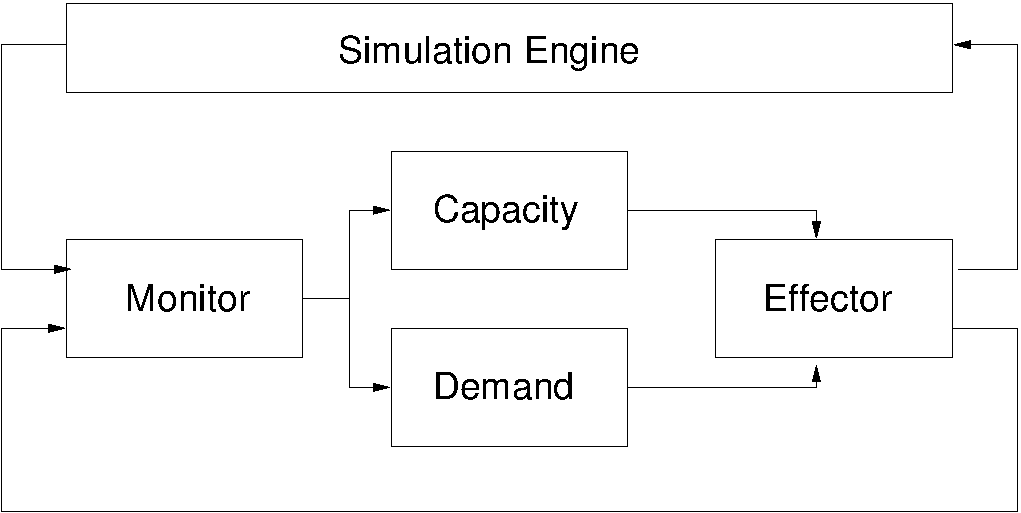
\includegraphics[scale=0.5]{../monograph/images/extension-block.pdf}	
	\end{figure}
\end{frame}